\renewcommand{\rmdefault}{ptm} % Arial:phv, Roman:ptm
\renewcommand{\sfdefault}{ptm} % Arial
\documentclass[journal]{IEEEtran} % onecolumn,12pt
\hyphenation{op-tical net-works semi-conduc-tor}



%\usepackage{program}

\usepackage[caption=false,font=footnotesize]{subfig}
\usepackage{xcolor}
\usepackage{color}
\usepackage{cite}
\usepackage{amsmath}
\usepackage{amssymb}
\usepackage{amsthm}
\usepackage{graphicx}
\newtheorem{theorem}{Theorem}
\newtheorem{prop}{Proposition}
\newcommand{\indep}{\rotatebox[origin=c]{90}{$\models$}}
\usepackage{epstopdf}
\usepackage{comment}
\usepackage{multirow}
\usepackage{algorithm2e}
\usepackage{threeparttable}
\usepackage{booktabs}
\usepackage{multirow}
\usepackage{amsmath}


%\usepackage[switch,right]{lineno}
%\linenumbers

\graphicspath{{./Pictures/}}



\definecolor{orange}{rgb}{1,0.5,0}


%\linespread{2}

\begin{document}
\title{Distribution Expansion Cost Allocation Algorithm Based on Stochastic Cooperative Game Theory and Long-Term Forecasting with Gibbs Sampling}

\author{Wonseok~Choi,~\IEEEmembership{Student Member,~IEEE,} ~Hyeonjin~Kim,~\IEEEmembership{Student Member,~IEEE,}
	Duehee~Lee,~\IEEEmembership{Member,~IEEE,}
	}





% The paper headers
\markboth{IEEE Transaction on Power System}
{Shell \MakeLowercase{\textit{et al.}}: Bare Demo of IEEEtran.cls for Journals}
\maketitle



\begin{abstract}
\textcolor{blue}{We propose the distribution expansion cost allocation algorithm based on the long-term load and renewable energy scenario forecasting. For the distribution expansion, the fluctuation of distributed electricity load and renewable energy sources (RES) should be particularly considered to allocate costs based on maximum power flows and their profits. We reflect the spatio-temporal correlations of distributed long-term load and RES into the probabilistic distributions of future scenarios from multiple nodes through the Gibbs sampling.
%
We sample future weather scenarios from multivariate distributions of temperature and dew point from eight weather stations. We convert the weather scenarios into the load and RES distributions by using the hierarchical graphical model. 
%
Currently, the costs are allocated among stakeholders based on averaged durations of maximum power flows, so the allotment cannot be linearly proportional to the expected profits and distribution usages. Therefore, we allocate the costs by using stochastic cooperative game theory based on long-term scenarios. Besides, we detect and remove a trigger project, which extremely increases the overall expansion cost.
%
We verify our algorithms by using the data from the Global Energy Forecasting Competition 2017. For forecasting performance, our approach outperforms the benchmark in the competition. Allocated costs depend on profits obtained from the transmission expansion, so our allocation algorithm is justifiable.}
\end{abstract}



% long-term forecasting and cost allocation

%The results of SCGT are averaged based on the fuzzy weighted average (FWA) theory.



% Therefore, the cost allocating of existing methods does not accept this volatility, so it could cause irrationality if applied to current network.

%Distributions are combined to build the final distribution through the advanced kernel density estimation. 


% Such benefit calculation result in discrete representation of stochastic benefit associated with time for each period, and by substituting this for SCGT


% muiltiple node
% stakeholders

% We allocate transmission expansion costs among stakeholders based on the long-term hourly electricity load forecasting from multiple nodes. 

%Since we cannot obtain the numerical weather prediction in far future, we forecast the probabilistic distribution of hourly load. 


% We calculate the expansion costs based on the power transfer distribution factors, which are calculated with future load scenarios on each transmission line. The cost are allocated through the cooperative competition among stakeholders.



% Quantile Regression
%we first make a demand map according to confidence interval through quantile regression using Gibbs sampling  Quantile regression allows us to calculate the utility benefits  by outputting discrete probabilistic demand distribution over time. 


%  However, the higher penetration ratio of renewable energy in distribution, the higher volatility of demand. 


% In case of distribution, expected demand of each consumption zone was determined and contribution calculated.

% Common network expansion cost, including general distribution, are allocated by mathematically calculating contribution of the line. 


	
\begin{IEEEkeywords}
Gibbs sampling, Stochastic cooperative game theory, Distribution network expansion plan, Cost allocation
\end{IEEEkeywords}
	
	
	
	

% \IEEEPARstart{T}{he} 
\section{Introduction}
% --------------------- Currnet Status ------------------------------
% --------------------- Why we have to forecast the load? 

\subsubsection{Current}
\textcolor{teal}{The distribution should be expanded to accept the pear-to-pear transaction, distributed generated renewable energy sources (RES), and storage systems. Grid-modernization is weighted and RES penetrates into distribution, that is a post-transmission in decentralized form. In the past, consumers were simply main users of electricity in electricity market, and in the current energy market, where RES penetrated, they were placed in compatible position to produce and sell energy. Since existing unidirectional network cannot accomdate this compatible energy flow, it is necessary to expand new distribution to enable two-way energy flow.}

% 각각 3가지에 대해서 왜 새로운 GRID mordenization 상황에서 배전망 업그레이드가 필요한지 적자.

\vspace{1in}





















% 전통적인 distribution 또는 내용을 찾기 힘들면 transmission의 확장 방법
% 전통적인 distribution expansion plan을 통해서 수요와 신재생에너지 예측이 필요하다는 것을 도출한다.
\subsubsection{Distribution Expansion Plan}
\textcolor{magenta}{Generally, the distribution expansion plan can be scheduled to satisfy the maximum load flows.
%
%
%
%
%
%
%
%
%
Then, we have to perform the long-term load and RES forecasting.}








\vspace{1.2in}














% 3-5가지 long-term load forecasting 방법 적고 비판
% 단순히 3-5가지 아무 방법을 언급하는 것보다는 적용 사례 3-5가지를 적고, 사례별로 내려가는 게 좋을 듯. 거기다 기술들이 나온 시간 순서도 고려해서.
% short 나 middle 들어가지 않고 바로 long. 필요하면 short나 middle은 한 두 문장 정도로 요약
\subsubsection{Long-Term Load Forecasting}
\textcolor{gray}{There have bee much research about long-term load forecasting.}


%%  ------------   About the forecasting duration.--------------------
Long-term forecasting covers the load forecasting for three years or more. Normally in long-term forecasting, in order to reflect the effect of human activity on the load in the future, the effects of economic growth should be considered~\cite{Tao2014}. 






% 예비력 정도는 long-term 사례로 적어도 되겠다.
For example, the required amount of ancillary services should be estimated a month ahead based on load forecasts, so short-term forecasting is not a proper approach for forecasting load, and long-term forecasting is not as accurate as mid-term forecasting. Furthermore, mid-term load forecasting is required to prepare unit commitment and maintenance schedules a month ahead of time based on the load forecasts~\cite{burger2014managing}.





% 원래는 mid-term에 대해 적힌 내용인데 long-term에 대해서도 적자.
%% ----------Why is the Long-term forecast complex-------------------
While mid-term forecasting has many benefits, mid-term load forecasting is the most complex. Ordinary load forecasting models use NWP which includes weather variables like temperature, humidity, data, and time~\cite{xie2016temperature} that affect humans' load usage. If NWP data exists, the load can be predicted using the relationship between the NWP and the load~\cite{bacher2013short}. However, NWP can only produce effective results when used for forecasts of up to two weeks. So, it is difficult to use NWP data for mid-term load forecasting. 
%%-------------------------------------------------------------------




%%--------- The method when existing method cannot use---------------
When NWP data is unavailable, time series models have been used to forecast loads recursively~\cite{TIMESERIES}. Another method involves estimating future NWP scenarios from the historical weather data, and using these scenarios to predict future load~\cite{xie2016temperature}. 







\subsubsection{Probabilistic Load Forecasting}
\textcolor{cyan}{In order to overcome the low accuracy of long-term load forecasting, generally the probabilistic load forecasting methods have been used to provide the probabilistic distribution of load forecasts.}


Recently, probabilistic load forecasting has been proposed to circumvent unavailable NPW~\cite{xie2016temperature}. In probabilistic load forecasting, future NWP scenarios are synthesized and converted to future load scenarios, and then, point forecasts can be made based on the mean or median of the marginal distribution of the future load scenarios.
%%------------------------------------------------------------------







%% ------------------------ Generating Scenario -------------------------
There is much literature about mid-term probabilistic load forecasting. One way to synthesize NWP scenarios is to reuse the historical data. In~\cite{Tao2014}, ten years of the historical temperature data was used to generate 10 different temperature scenarios, which were then used to predict 10 different load forecasts. However, only a limited number of scenarios can be obtained from historically measured data, and this will reduce forecasting accuracy. In~\cite{Jingrui2015}, to increase the number of scenarios, forecasting errors were collected by comparing the predicted values with the actual values. The errors were modeled as a normal distribution, where an infinite number of scenarios can be sampled.  Many participants at global energy forecasting competition  (GEFCom) 2017 used an hourly sampling method to synthesize temperature scenarios~\cite{hong2019global}. 


\vspace{1in}







% 확률 예측을 위한 sampling 방법에 대해 공부
% spatio-temporal 관련된 내용을 공부하자.
% 일단 시간 축에 대한 sampling이 필요하다.
% 그리고 공간에 대한 sampling이 필요하다.
% 각각의 경우에 대해 sampling 하는 사례를 적고, 둘다 sampling 하는 경우도 적자.
\subsubsection{Sampling}
\textcolor{red}{Future load can be converted from future weather scenarios, which can be sampled from multivariate distributions of different weather variables and locations.}



\vspace{1in}



However sampling from one-dimensional distribution cannot consider relative humidity (RH) which has a significant effect on load forecasting~\cite{xie2016relative}. 

Also~\cite{xie2017variable} showed that the hourly or daily ahead data for temperature can be used to improve the preciseness of load forecasting. But, hourly samples cannot consider the joint probability between samples of different times. Also using hourly independent samples, matching time ahead data might deteriorate the correlation between features.  
%%












\subsubsection{Point Forecasting XGBoost}
\textcolor{cyan}{Although we cannot expect an accurate point value in the probabilistic forecasting, the fast and accurate enough algorithm is still necessary to convert future weather scenarios into load forecasts.}



\vspace{1.3in}

































\subsubsection{Detecting Triggering projects}
\textcolor{orange}{After the distribution expansion plan is scheduled based on long-term forecasts, in particular, the distribution expansion is a radial network, so there could be an expansion plan, which locates in a bottle neck and causes extremely high expansion costs. If we can remove that plan or allocate the cost into stakeholders, we can expedite expansion and reduce the total expansion cost. }





\vspace{1in}







\subsubsection{Cost Allocation}
\textcolor{olive}{The cost of a scheduled distribution expansion plan should be allocated to stakeholders. There have been several studies on the transmission expansion cost allocation.}



\vspace{1in}







%-----------------------------------------------------------------------

%% --------------------    Averaging the distribution -------------
%%Second, the quantile regression algorithm can be used to estimate quantiles of the error distribution. If the first and second methods are combined, the quantiles of many load scenarios are averaged to generate the final load quantile. In~\cite{Gaillard}, the error distribution of each temperature scenario is obtained through the quantile generalized additive model, which is also known as an ensemble model. The error distributions from 800 temperature scenarios are averaged to estimate a single final error distribution of the future load. However, the averaged temperature scenario, which is the uniform weighted average of temperature from 25 weather stations, is used. If all temperature scenarios from 25 weather stations are used, a better performance might be obtained because sufficient information of 25 temperature scenarios could be utilized.

%%%%% ----------------- Probabilistic Forecast without scenarios. -----------------
%%Furthermore, the temperature scenarios are not necessary factors to forecast the error distribution of the load forecast. In~\cite{Bidong}, Liu et al used the concept of sister models and their forecasts to forecast the error distribution. Individual forecasting models, which are called sisters, forecasted their own forecasts by selecting different variables and features. Finally, the quantile regression was used to estimate the error distribution of the sister forecasts. However, using the multiple forecasts of multiple forecasting models might result in a deterioration of the overall forecasting accuracy because the best performing model as well as inaccurate models are combined.


%% ------------------------ KDE --------------------------------
%%




















\subsubsection{Task}
In this study, we develop an advanced algorithm for mid-term probabilistic load forecasting. First, as mentioned above, many studies used a one-dimensional temperature scenario, whereas we sample the interrelated temperature and dew point  scenarios from their multivariate Gaussian distribution (MGD). In this process we also consider the daily patterns and dependency between hourly weather data using joint distribution of hourly random variables. %%We compare the performance between our method to the single dimensional scenarios and also the  historical scenarios.

Second, we propose a probabilistic graphical model (PGM) which can provide an intuitive graphical model of the joint probabilities when considering a problem. PGM can visualize dependency and relationships between random variables and simplify marginal probability.

Third, we use Gibbs sampling. In the case of MGD, general sampling method is difficult to converge for a specific purpose in a multi-dimension distribution, and it is not possible to consider the dependency between variables. Therefore, we use Gibbs sampling in this paper to solve above problems.

Fourth, we use the extreme gradient boosting model (XGBoost). XGBoost is the ensemble algorithm that uses a combination of several decision trees. XGBoost has both performance and resource efficiency, so it is one of the most popular forecasting algorithms. XGBoost is an improvement on the gradient boost machine (GBM), and it uses several low accuracy forecast models rather than a single high accuracy model like GBM.   

Fifth, We use kernel density estimation (KDE) for post-process which can generate smooth non-parametric distribution for hourly load from load scenarios which can preserve each observation. Also by using KDE we can get a mathematical form of load PDF which can be utilized in many different ways for power system problems. In this process we set the bandwidth parameter by forecasting residuals in the cross validation process which can substitute residual simulation.

Finally, we present a method of cost-allocation among utilities using cooperative game theory (CGT) to show the utilization of mid-term forecasting in electricity system planning based on the provided demand forecasts.
 
%Third, we propose a better way to structure the hierarchical forecasting problem by comparing the performance of several models. PGM can visualize dependency and relation between random varibles and simplify marginal probability that we are considering as mulipilication of several conditional probability. Fifth, we choose weather stations by gamma test simulation. 
%% a result of   find the optimal length of days and hours collecting samples to maximize the forecasting performance. The multivariate distribution of scenarios can only be estimated through historical measurement. Therefore, we expand the length of days to collect temperature samples, but we keep the characteristics of temperature on the target day. 

% Third, the kernel density algorithm (KDA) can be used to estimate the distribution of loads by assuming that there is a prior distribution for the load or NWP. If the prior distribution has a closed form, it is called the parametric approach, but if it does not, it is called the non-parametric approach. For example, in~\cite{Mangalova}, the error distribution of the load was found using the non-parametric kernel density method.
%% ---------------------------------------------------


%% The contents of this paper are as follows. In Section $\rm{2}$, we introduce the forecasting environment and the data used to verify our algorithm. In Section $\rm{3}$, we introduce probabilistic graphical model and propose the graphical model of load forecasting problem and NWP scenarios are estimated by the Gibbs sampling. In Section $\rm{4}$, the XGBoost is introduced. And marginal load distribution is estimated by the kernel density estimation.In Section $\rm{5}$ we measure the performance of several forecasting techniques and compare the performance of different forecasting structures with that of the proposed algorithm. Finally, Section $\rm{6}$ summarizes the contents.
%% -----------------------------------------------------------------------------------------------------------------







\subsubsection{Contribution}

Our contributions are as follows:
\begin{enumerate}	
	\item We synthesize future WPG scenarios with the same statistical characteristics of actual WPG.
	\item We develop a novel PSD estimation method to reduce the PSD variance.	
	\item We model a novel flexibility index that can consider the long and short-term variability of WPG.	
	\item We develop a recursive algorithm that can calculate the optimal amounts of flexible resources.
	\item We measure the value of the smoothing effect as a function of the total wind power capacity.
\end{enumerate}


























\newpage
\section{Distribution Expansion Cost Allocation Algorithms}




\subsection{Distribution Expansion Planning}






\subsection{Traditional Cost Allocation Algorithms}






\newpage
\subsection{PJM Expansion Protocol}





\subsection{Triggering Expansion Project}


















































\newpage

\section{Scenario Generation}

%% 1. Data Explanation
In this section graphical modeling and Gibbs sampling are introduced. Observed temperature and dew point are designed as a MGD based on the graphical modeling, and their scenarios are synthesized based on the Gibbs sampling.



%A series of events or a system are represented by variables and observed by measurement of variables, and a distribution of multiple measurements is represented by a multivariate distribution of variables. 

% The conditional independency is very useful when only few variables in a multivariate distribution are observed.}  

%We can think of directed graph as a filter that allows a distribution to pass through if it can be expressed as the factorized implied. 



% Necessity of graphical modeling: Simplify the full joint distribution by using the conditional dependency



%In order to represent the multivariate distribution, parameters to represent the dependencies among variables should be specified, so the more variables are in the distribution, the more parameters are specified. 


\subsection{Forecasting Environment and Data Description}

%%%%%%%%%%%%%%%%%%%%%%%%%%%%%%%%%%%%%%%%%%%%
In this study, the load is forecasted by following the forecasting environment of the GEFCom 2017. The distributions of month-ahead load from 10 zones should be forecasted at every hour for 31 days upto two month ahead. The distribution is represented by nine quantiles from 10\% to 90\% at every 10\%. 


Furthermore, from the GEFCom 2017, the historical load from eight zones and historical weather observations from eight weather stations are provided. These data were hourly measured for 14 years. Historical weather observation consists of temperature and dew point. It should be noted that all training data is measured data, so the NWP is not used. 

A historical load was measured from eight zones in the New England independent system operator (ISO-NE). Eight zones are New Hampshire (NH), Vermont (VT), Rhode Island (RI), west central Massachusetts (WCMA), south-east MA (SEMA), north-east MA (NEMA), Connecticut (CT), and Maine(ME). In addition to eight zones in ISO-NE, the entire ISO-NE is considered as a hierarchical structure total load.

%% Tradining data info
The training set consists of the weather and time data. As mentioned above the weather data includes temperature and dew point, and the time data includes year, month, day, and hour. 

%% Forecasting models.
The 8 different forecasting models predict the load of 8 zones in parallel manner. Because no weather station is representative for ISO NE and total MA zone thus we added forecasted values underlying each hierarchical structures. 

For training set and NWP scenarios, selection of weather station is determined by gamma test. Selected weather stations for each zone consist of joint MGD and Gibbs sampling through Probabilistic Graphical Model is utilized to generate target input stream which is NWP scenarios.

 %%We verify our method by forecasting the load of ISO NE on march, 2017 and this was target period of round 5 on GEFCom2017. The forecasting architecture including every sequences on our research is represented in Fig~\ref{ForArchi}, also weather station on each zone is represented in Fig~

 In this paper, the performance of distribution is evaluated by the pinball loss function. The pinball loss in~\cite{Hong2016} is used to measure the performance of probabilistic forecasting when the distribution is represented as quantiles. The loss function is defined as:
\begin{equation}
L({q_a},y) = \left\{ {\begin{array}{*{20}{c}}
  {(1 - \frac{a}{{100}}) \times ({q_a} - y)}&{if\,y < {q_a}} \\ 
  {\frac{a}{{100}} \times ({q_a} - y)}&{if\,y \geq {q_a}},
\end{array}} \right.
\end{equation}
where $a$ represents a quantile percentage, $q_a$ represents the quantile prediction, and $y$ represents the target value.




%%%%%%%%%%%%%%%%%%%%%%%%%%%%%%%%%%%%%%%%%%%%%%%%%%%%%%%%%%%%%%%%%%
\subsection{Probabilistic Graphical Modeling}
%%% What is the graphical model

%% Definition of the graphical model
The  graphical model represent the multivariate probabilistic distribution as a network graph of nodes and edges. 
% Graph Component Explanation
The nodes represent variables in the multivariate distribution, and the edges represent the dependency between nodes. The direction of an arrow in an edge represents a dependency. Suppose there are two variables $A$ and $B$. If an edge has an arrow from $A$ to $B$, $B$ depends on $A$. By following arrows in a network, we can build the joint distribution. For example, starting from a root $A$ with a priori probability $p(A)$, we can build the conditional probability of $B$ with respect to $A$ as $p(B|A)$ by following an arrow. Then, we can build the joint distribution $p(A,B)$ over the variables $A$ and $B$ as the product of $p(B|A)$ and $p(A)$. In other words, in a network, a multivariate distribution can be decomposed by a multiplication of a few conditional probabilities by following arrows. Finally, the probabilistic model in a network helps us to sample scenarios.  



%% ----------------- Necessity of graphical modeling  -------------------------
The graphical model provides Three strong advantages to handle multivariate distributions.
%% 1. Simple way to visualize: Only use dependent variables.
% In a network, a distribution can be described as few parameters. 
First, it provides a simple way to visualize the structure of a probabilistic model since it is easy to detect the conditional independency through the network. For example, when a series of events occurs in sequence, the graphical model can represent a probability of the last event with respect to the probabilities of only dependent events. Second, since a network represents only the dependent variables, less number of parameters is required than a full description of distribution. On the contrary, without the graphical model, the probability of the last event should be represented by the probabilities of all beforehand events.
%% 2. Conditional independency 
Third, we can utilize the conditional independency. For example, in our application, if we know the date, the temperature from two different zones on the same date are independent. It is called a conditional independency. Since there is no strong reason that the temperature from different zones depend each other, we can assume that temperature is independent on the condition of the given day. By utilizing this conditional independency, we can simply multiply the probability of temperature and dew point. 


  
  



%% 2. Product of conditional probabilities

%When the first arrow represents a starting conditional probability, the next arrow represents the conditional dependency of a target variable and all previous variables, and these connectivity represents as a multiplication in a mathematical formulation. 



%%% ------------------   In our Case ------------------------------------
In our application, we use the graphical model to design the multivariate distribution of load and training data and sample future scenarios of temperature and dew point from the multivariate distribution. For our application, the temperature and dew point temperature depends on a month of year, and temperature and dew point have dependency on each other on given month. With a pair of temperature and dew point temperature we can derive a relative humidity which is not observed. Based on the reasonable inference, we can deduce a network graph from a given multivariate distribution. A multivariate distribution using graphical model that we considered is plotted in Fig~\ref{Dependency}. With graphical model we sampled multiple temperature and dewpoint scenarios depend on given month and time. Using two variables, temperature and dew point, we formed the multi probabilistic distribution.

  
  
  





\begin{figure}[t!]
\centering
  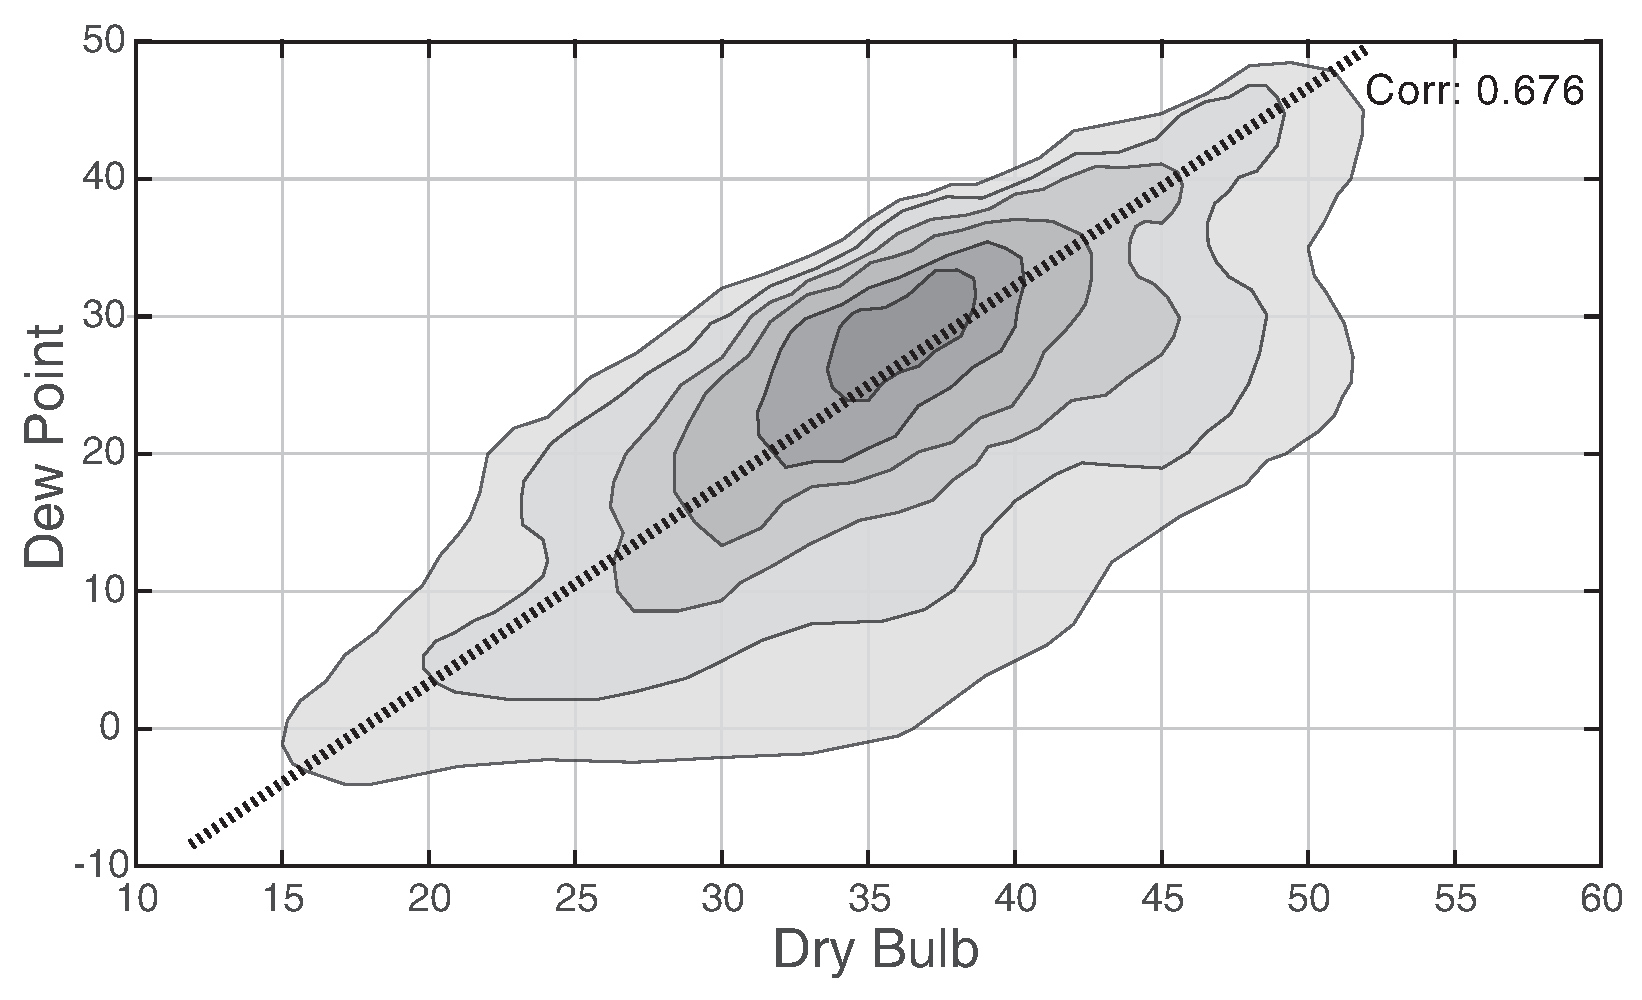
\includegraphics[width=3.5in]{Contour_AI}
\caption{Non-parametric bivariate distribution of dew point and dry bulb is represented. Two random variable show high correlation, which makes  weather scenario generation from joint density of these variable more convincing.}
\label{Dependency}       % Give a unique label
\end{figure}




%%
% We need samples to estimate the probabilistic distribution of future load. Samples can be generated from the inverse of cumulative distribution. Normally, samples are generated from a distribution to calculate the expectation of given function based on that distribution, but in our application, we only need samples to estimate the distribution of future electricity demand. However, the computational complexity increases as the number of dimension increases. Since we can generate arbitrary many number of samples, the network graph is a generative model.








%%%%%%%%%%%%%%%%%%%%%%%%%%%%%%%%%%%%%%%%
%%%%%%%%%%%%%%%%%%%%%%%%%%%%%%%%%%%%%%%%
%%%%%%%%%%%%%%%%%%%%%%%%%%%%%%%%%%%%%%%%
\subsection{Historical data collection for scenario generation}
%%%% Situation %%%%
The probabilistic model can be estimated from observation. We have temperature and humidity data from 8 different zones for 14 years. However, at the given day of year and hour, there are not many samples to build the probabilistic model. Besides, for the multivariate distribution, more samples are required to describe the distribution. 

%%% Collecting %%%
Therefore, we collect data for a few hours ahead and a few hours later. At the same time, we collect data for a few days ago and a few days later. The way to estimate accurate time and day spans were studied in~\cite{xie2016temperature}. We collected dewpoint and drybulb three hours ahead and after from each 14 years of historical data. A similar study for our application should be performed in future work.













%%--------------------------------------------------------------------------
%%%%%%%%%%%%%%%%%%%%%         Gibbs Sampling           %%%%%%%%%%%%%%%%%%%%%%
%%--------------------------------------------------------------------------

%%%%%%%%%%%%%%%%%%%%%%%%%%%%%
%% Sampling Techniques



\subsection{Gibbs Sampling}
In this study, the Gibbs sampling is used to sample sets of temperature and dew point for each zone. The Gibbs sampling is a kind of Markov chain Monte Carlo (MCMC) sampling algorithm, and it can also be seen as a special case of the Metropolis-Hastings sampling algorithm~\cite{Bishop} . As well as the Gibbs sampling, there are several sampling techniques in a graphical modeling: ancestral sampling, importance sampling, likelihood-weighted Sampling, logic sampling, Rao-Black wellisation, and Gibbs sampling. Among these techniques, the Gibbs sampling is used in our application since it is simple and fast~\cite{Gibbs}.


%%% Key idea of gibbs sampling
The main idea of the Gibbs sampling is as follows. Since it is difficult to sample a set of variables from a multivariate distribution, we can sample each target variable from the conditional distribution of a target variable with holding the others constant. After a variable is sampled, we will sample the next variable based on other sampled variables. In other words, we sample $x_1^{(j + 1)}$ from $\pi (x_1^{(j + 1)}|x_2^{(j)},x_3^{(j)}, \ldots ,x_d^{(j)})$. Then, we sample $x_2^{(j + 1)}$ from $\pi (x_2^{(j + 1)}|x_1^{(j+1)},x_3^{(j)}, \ldots ,x_d^{(j)})$. It should be noted the index of each variable. Finally, if we continuously sample variables one by one, the set of samples will follow the joint distribution. In this process, we assume that the dependence of samples follows a Markov chain, since the Gibbs sampling is a kind of MCMC sampling algorithm. 

 

 
 
The advantage of using the Gibbs sampling shed when the high-dimensional full joint distribution is not represented analytically, but the conditional distribution is simply described. Besides, if other variables are independent to a target variable, we can simply the conditional distribution, and it becomes a low-dimensional conditional distribution with only related variables.


There are many variables from 10 zones, but we can reduce the number of variables in the conditional distribution through our graphical model. Therefore, we only need to build the Markov chain for each zone. Therefore, we secure the conditional independency between scenarios from different zones through the graphical model. The temperature and dew point scenarios in different zones are sampled individually under the condition of target time. For each zone, scenarios are synthesized together through the Gibbs sampling.
  



%% Whole process
The algorithm of the Gibbs sampling is described below. In this study, we want to sample from a joint distribution $P({\bf{x}}) = P({x_1},{x_2})$ where $x_1$ represents the temperature, and $x_2$ represents the dew point. We assume that $P({\bf{x}})$ follows the bivariate Gaussian distribution.
%%%
First, we initialize samples.
\begin{equation}
\label{Initialize}
{{\bf{x}}^0} = ({x_1^0},{x_2^0})
\end{equation}
Then, we sample $x_1$ while holing $x_2$ constant as an initial value.
\begin{equation}
\label{X1sample}
x_1^{(1)} \sim \pi (x_1^{(1)}|x_2^{(0)})
\end{equation}
Then, while holding $x_1$ as a sampled value, we sample $x_2$. 
\begin{equation}
\label{X1sample}
x_2^{(1)} \sim \pi (x_2^{(1)}|x_1^{(1)})
\end{equation}
It should be noted that this procedure can be generalized for arbitrarily many variables.
%%
In this study, we assume that the temperature and dew point follow the bi-variate Gaussian distribution. The conditional Gaussian distribution when the other variable is known is introduced as
\begin{equation}
\label{ConditionalDist}
\small
\begin{aligned}
\pi(Y|X = x) \sim N\left( {{\mu _Y} + \rho \left( {\frac{{{\sigma _Y}}}{{{\sigma _X}}}} \right)\left( {x - {\mu _X}} \right),\sigma _Y^2(1 - {\rho ^2})} \right).
\end{aligned}
\end{equation}
The joint Gaussian distribution is estimated from the observation of temperature and dew point.
%
These processes should be repeated for several times until the conditional dependency between variables are represented in samples, and the independency of initial values is disappeared. The processes can be summarized as an algorithm in the Algorithm~\ref{Gibbs}, where $N$ is the required number of samples, and $M$ is the number of iterations.
\begin{algorithm}[t!]
\label{Gibbs}
 \KwData{Temperature and dew point}
 \KwResult{$N$ sets of samples}
 \For{i:1 to $N$}{
 \textbf{Iinitialization\:} ${{\bf{x}}^0} = ({x_1^0},{x_2^0})$ \\
  \For{j:0 to $M$}{
    Sample\;
    $x_1^{(j+1)} \sim \pi (x_1^{(j+1)}|x_2^{(j)})$ \;
	$x_2^{(j+1)} \sim \pi (x_2^{(j+1)}|x_1^{(j+1)})$ \;
    Go to the next iteration\;	
    }
    Collect $({x_1^M},{x_2^M})$ \;
    Go to the next iteration\;	
   }
 \caption{The algorithm of the Gibbs Sampling }
\end{algorithm}






%%
 In this application, we assume that vectors of samples follow the multivariate Gaussian distribution.




\subsection{Scenario Generation}

In this section, we will generate temperature and humidity scenarios for target month. We considered multivariate joint distribution which is consisted of random variables of few different weather station's dry bulb and dew point temperature. Each dew point and dry bulb temperature is a vector of random variables which consist of 24 random variables that mean a variable for an each hour. Sampling NWP from this joint distribution can consider correlation between dry bulb and dew point temperature and this pair of data can be interpreted as relative humidity. The advantage our relative humidity on load forecasting is described in []. Temperature and humidity is continous in every moment thus sampling for each hour and combining them arbitrarily can break the pattern which has in nature. Through our method such pattern can be kept. This is important because considering preditors such as temperature of few hour ahead can improve forecasting performace which is written in[]. And if temperature scenarios which don't consider the correlation of each hour make awkward match in predictor set. For checking our sampling method, we considered sampling from other distribution. We made each distribution of DB and DP temperature considering hourly variable and randomly matched each sample and we call this as individual method. We also considered sampling from hourly distribution of DP and DB and this is hourly method. 



\section{Forecasting Methods}
In this section, the distributions of load forecasts are estimated for each scenario through two different methods, which are the qunatile regression of gradient boosting machine and the quantile regression of random forest. Then, the multiple distributions of scenarios for a single target case are combined through the kernel density estimation based on the Gaussian mixture model. Furthermore, The performance of the Gaussian mixture model is compared to the empirical method of distribution averaging. 





\subsection{Basic of Quantile Linear Regression}
In this subsection, we will introduce how to perform the quantile regression.

%% Definition of quantile
The quantile $y_q$ at the given percentage $q$ means the value of random variable whose cumulative probabilities become the given percentage. This can be represented as 
\begin{equation}
\label{QuantileDefinition}
{y_q} = {F^{ - 1}}(q)
\end{equation}
where $q$ represents the percentage, and $F$ represents the cumulative distribution function (CDF). 
%% Example
For example, the median is the 0.5 or 50\% quantile. Therefore, the quantile is the output of inverse CDF at the given percentage.




%% Definition of Quantiles.
We can start from a well known fact that the value, which can minimize the sum of absolute errors between samples, is the median. In short, the median has the least-absolute deviation (LAD). It is obvious that finding the median is a sorting and selecting problem. Since $P(X \le m) = P(X \ge m) = 0.5$, where $m$ is the median, the median is in the middle of sorted samples. Then, if we assume that we can only find a median, in order to find other quantile for different percentages, we can change the number of samples in the left hand side of quantile by multiplying a weight factor. For example, if we want to find the quantile at the 80 \%, we can multiply the coefficient 0.8 to the right hand side of quantile. This will make a virtual situation that we have many samples right hand side of quantile. Therefore, finding a median is to find the value of the LAD. Similarly, finding a quantile is to find the value of the LAD of weighted samples.


%%
By using this approach, we can find a quantile at a given percentage, which can minimize the sum of LADs. 
%% Least Square
Generally, the ordinary linear regression minimizes the sum of all losses, but the quantile regression minimizes the asymmetric penalties with different weight factors. When it is over-predicted, the $1-q$ is multiplied to the loss, and when it is under-predicted, the $q$ is multiplied to the loss. Then, the loss function becomes as
\begin{equation}
\label{QuantileLossFunction}
\begin{aligned}
L(y,{\beta _q}) & = q\sum\nolimits_{{y_i} > {{\bf{x}}_i}{\beta _q}} {({y_i} - {{\bf{x}}_i}{\beta _q})}  \\ & + (1 - q)\sum\nolimits_{{y_i} \le {{\bf{x}}_i}{\beta _q}} {({{\bf{x}}_i}{\beta _q} - {y_i})}
\end{aligned}
\end{equation}
where $\beta$ is the coefficient of linear regression.






The quantile regression represents the distribution of forecast as quantiles.




%% Comparision to the orginay regression
In the linear regression, it leads to the projection of solution vector onto the subspaces of observation data. On the contrary, in the quantile regression, it should be solved by techniques in the linear programming.





%%%%%%%%%%%%%%%    How to solve quantile regression     %%%%%%%%%%%%%%%%%%%%
If we know the CDF of a certain variable, we can get quantiles by inversing the CDF. However, if we only know samples, we can get quantiles by solving an optimization problem for the given samples. Moreover, the quantile regression can be considered as inversing the CDF if we can get the empirical CDF from samples.






\subsection{Quantile Regression of Gradient Boosting Machine}
The GBM is the most widely known a probabilistic regression tool~\cite{Friedman}. Several forecasting competition winners have been used this algorithm. 


%% Probabilistic Forecasting methods
There are two representative methods to forecast the distribution of forecasts: the quantile regression based on a specific forecasting algorithm and the estimation of distribution through analyzing forecasting errors. 
%
The second method estimates the error distribution by collecting forecasting errors. Errors are collected by comparing the actual values and forecasted values. 

%% Advantages of the GBM
However, the quantile regression can generate different distributions for the given weather conditions. In other words, the error distribution methods can have limited number of different distributions for different given observation data. On the contrary, quantile regression can have different variance for the given observation data. In other words, if the quality of the target observation data is bad, the variance of the distribution increases, but if the quality of the target observation data is good, the variance of the distribution decreases, and it means that we have a narrow and accurate distribution.


For the quantile regression approaches, the representative forecasting algorithms used in the quantile regression approaches are the GBM and the RF. In this study, we use both methods and compare their performance.

The problem of the quantile regression is that we should solve the same number of problems for the given number of quantiles. Furthermore, quantiles might not be sorted, so the CDF might not be non-increasing, then the PDF could be negative, which cannot happen normally.



%%%%%%%%%%%%%%%%%%%%%%%%%%%%%%%%%%%%%%%%%%%%%%%%%%%%%%%%%%%%%%%%%%
%%%%%%%%%%%%%%%%%%%%%%%%%%%%%%%%%%%%%%%%%%%%%%%%%%%%%%%%%%%%%%%%%%
In this study, we define the "training set`` as a combination of "$N$ training data" $ \bf{X}=\left\{ {{{\bf{x}}_1}, \ldots ,{{\bf{x}}_N}} \right\}$ and the "$N$ target values`` $\bf{y} = \left\{ {{y_1}, \ldots ,{y_N}} \right\}$. The goal of the forecasting is to estimate the function $\hat{F}(\bf{X})$, which can approximate the actual function $F(\bf{X})$ so that ${\bf{y}} = F(\bf{X})$. The $\hat{F}(\bf{X})$ can be estimated to minimize the sum of loss function $L({\bf{y}}, F(\bf{X}) )$ over the combination of $( {\bf{y}}, {\bf{X}})$. Then, the $\hat{F}(\bf{X})$ can be found by solving a simple minimization problem
\begin{equation}
\label{GBMobject}
\hat F({\bf{X}}) = \arg \,\mathop {\min }\limits_F \,\sum\limits_{i = 1}^N {L({y_i},F({{\bf{x}}_i}))}.
\end{equation}

In the GBM, this minimization problem is solved by three key ideas.
%% Key Idea of the GBM
The first key idea of the GBM is that we can present the $\hat{F}(\bf{X})$ as the sum of several functions $f_m({\bf{X}})$ as 
\begin{equation}
\label{SubFunctions}
\hat F({\bf{X}}) = \sum\limits_{m = 1}^M {f_m({\bf{X}})}, 
\end{equation}
where $f_m({\bf{X}})= b_m h({\bf{X}}; {\bf{a}}_m)$ under the assumption that all $f_m({\bf{X}})$ have the same basis function $h({\bf{X}})$~\cite{Tibshirani}.


Then, the second key idea, which is a strategy to find $\hat F({\bf{X}})$, is to update it by finding $b_m h({\bf{X}}; {\bf{a}}_m)$ as
\begin{equation}
\label{Update}
{F_m}({\bf{X}}) = {F_{m - 1}}({\bf{X}}) + {b_m}h({\bf{X}};{{\bf{a}}_m})
\end{equation}
where $h({\bf{X}};{{\bf{a}}})$, which is a basis function with known parameters, is called a weak learner.
%%
The $(b_m,{\bf{a}}_m)$ can be obtained by solving
\begin{equation}
\label{Parametric}
({b_m},{{\bf{a}}_m}) = \arg \mathop {\min }\limits_{b,{\bf{a}}} \sum\limits_{i = 1}^N {L({y_i},{F_{m - 1}}({{\bf{x}}_i}) + bh({{\bf{x}}_i};{\bf{a}}))}.
\end{equation}

The updating component ${b_m}h({\bf{X}};{{\bf{a}}_m})$ in (\ref{Update}) can be found through the steepest descent approach~\cite{AAA}, where $h({\bf{X}};{{\bf{a}}_m})$ is defined as the gradient of the loss function as
\begin{equation}
\label{Gradient}
{g_m}({{\bf{x}}_i}) = \left[ {\frac{{\partial L({y_i},F({{\bf{x}}_i}))}}{{\partial F({{\bf{x}}_i})}}} \right].
\end{equation}
However, the problem of this approach is that the gradient is obtained only for the observation data $\bf{x}$.
%% Smooth
The solution of this problem is to find the smooth functoin $h({\bf{X}};{{\bf{a}}_m})$ so that we have values for unknown observation $\bf{x}'$. One of good smooth basis function is a decision tree~\cite{WWW}, and we will also use a decision tree in this study. Then, what we have to do is to find parameters ${\bf{a}}_m$ so that $h({\bf{x}_i};{{\bf{a}}_m})$ has a similar values to ${g_m}({{\bf{x}}_i})$. However, since it is difficult to find $b_m$ and ${\bf{a}}_m$ simultaneously, we will find ${\bf{a}}_m$ first for the given $b_m$ and find $b_m$.
%% Finding a
The ${\bf{a}}_m$ can be found by solving the next minimization problem
\begin{equation}
\label{Afinding}
{{\bf{a}}_m} = \arg \mathop {\min }\limits_{b,{\bf{a}}} \sum\limits_{i = 1}^N {{{\left[ { - {g_m}({{\bf{x}}_i}) - bh({{\bf{x}}_i};{\bf{a}})} \right]}^2}}
\end{equation}
This is a simple regression tree generation. Then, 
\begin{equation}
\label{Bfinding}
{b_m} = \arg \mathop {\min }\limits_b \sum\limits_{i = 1}^N {L({y_i},{F_{m - 1}}({{\bf{x}}_i}) + bh({{\bf{x}}_i};{{\bf{a}}_m}))}
\end{equation}
Finally, we could estimate a set of $({b_m},{{\bf{a}}_m})$.





%%%%%%%%%%% How to provide the error distribution
These all processes depend on the loss function. For example, if the loss function is a simple least-square loss function, which is defined as  
\begin{equation}
\label{LeastSquare}
L(y,F) = \frac{{{{\left( {y - F} \right)}^2}}}{2},
\end{equation}
then the gradient can be simply calculated as 
\begin{equation}
\label{LSgradient}
{g_m}({{\bf{x}}_i}) = {y_i} - {F_{m - 1}}({{\bf{x}}_i})
\end{equation}


%%%% Quantile Regression
In this study, we should use the quantile loss function, which is defined in~\cite{Ridgeway} as
\begin{equation}
\begin{aligned}
\label{QuantileLossFunction}
L(y,F)&  = \alpha \sum\nolimits_{{y_i} > f({{\bf{x}}_i})} {({y_i} - F({{\bf{x}}_i}))}  \\ &  + (1 - 1\alpha )\sum\nolimits_{{y_i} < f({{\bf{x}}_i})} {(F({{\bf{x}}_i}) - {y_i})}
\end{aligned}
\end{equation}
where $\alpha$ represents the quantile range, i.e. 0.1 represents 10\%. Then, the gradient can be obtained as
\begin{equation}
\label{QuantileGradient}
{g_m}({{\bf{x}}_i}) = \alpha {\bf{I}}({y_i} > f({{\bf{x}}_i})) - (1 - \alpha ){\bf{I}}({y_i} \le f({{\bf{x}}_i}))
\end{equation}
%% Forecasting
Finally, when the GBM forecasts the future value for new data, GBM generates outputs by adding results of all basis functions.







% 1. Using the GBM

% 2. Using the Bag

% 3. Using the general approach changing objective function



%Meinshausen, N. "Quantile Regression Forests." Journal of Machine Learning Research, Vol. 7, 2006, pp. 983?999.




\subsection{XGboost}

















\newpage
\subsection{Kernel Density Estimation}
In this subsection, we will find the final list of quantiles by combining lists of quantiles from scenarios. We use the kernel density estimation (KDE) with a Gaussian kernel. The Gaussian mixture model is a popular way to estimate the multi-modal distributions, which has multiple peaks when we have several distributions of different shapes~\cite{Haben}. Besides, by building a final list of quantile, we can have a non-decreasing list of quantiles. We also build the final list of quantiles by simply collecting samples from each list of quantiles. 




%%%% Gaussian Mixture Model
The Gaussian mixture model (GMM) is another way to combine several distributions. It is similar to the KDE, where all points have a same small distribution. On the contrary, in the GMM, several Gaussian distributions with different means and variances are fitted to samples, and the number of distributions should also be estimated. In this application, since each quantile does not follow the Gaussian distribution, the GMM might not fit to our application.





%%%%%%%%% KDE Formulation %%%%%%%%%%%%
The basic idea of the KDE in~\cite{Duda} as follows. In the KDE, the probability density of a new random variable $x$ is measured by adding all numbers of samples within the fixed range around $x$. The number of samples $K$ can be calculated as
\begin{equation}
\label{K}
K = \sum\limits_{n = 1}^N {\kappa  \left( {\frac{{x - {x_n}}}{h}} \right)},
\end{equation}
where $N$ is the number samples, $x_n$ is the $n$th sample, $\kappa$ is the kernel function of counting, and $h$ is the smoothing parameter. The $h$ trades off between the variance and bias~\cite{Bishop}. A large $h$ leads to a very smooth distribution, but a small $h$ leads to a noisy distribution, where each variable has a peak in the worst case.
%%
It should be noted that $x$ is a scalar variable. By normalizing it, we can get the probability density of $x$ as
\begin{equation}
\label{K_PDF}
p(x) = \frac{1}{N}\sum\limits_{n = 1}^N {\frac{1}{{{h^D}}}\kappa \left( {\frac{{x - {x_n}}}{h}} \right)},
\end{equation}
where $D$ is the dimension of data, so it is one in this application.
%%% Gaussian Case
When the kernel function is a Gaussian distribution, the marginal probability over samples is defined as
\begin{equation}
\label{GaussianCase}
P(x) = \frac{1}{N}\sum\limits_{n = 1}^N {\frac{1}{{\sqrt {2\pi {h^2}} }}\exp \left\{ { - \frac{{{{\left\| {x - {x_n}} \right\|}^2}}}{{2{h^2}}}} \right\}}
\end{equation}
%%%%% Kernel Density Method
Therefore, the final list of quantiles is obtained by placing a Gaussian over each sample and adding distributions over all samples. The sum of distributions should be normalized by dividing the number of all samples.


%\textbf{The bandwitdh acts as a smoothing parameter, controlling the tradeoff between bias and variance. A large bandwidth leads to a very smooth density distribution, but a small bandwidth leads to an unsmooth density distribution.}



In order to test the performance of the KDE, we just simply generate the final density of forecasts by adding a single quantile from each scenario. The final quantile can be generated from a quantile of each scenario. For the given adjacent two quantiles among nine quantiles from 0.1 to 0.9, we can generate uniformly distributed samples. Then, we can have samples from the given list of quantiles. If we collect all samples from all lists of quantiles. For the collected samples, we can re-build a list of quantiles from 0.1 to 0.9.

%\begin{figure}[t!]
%\centering
%  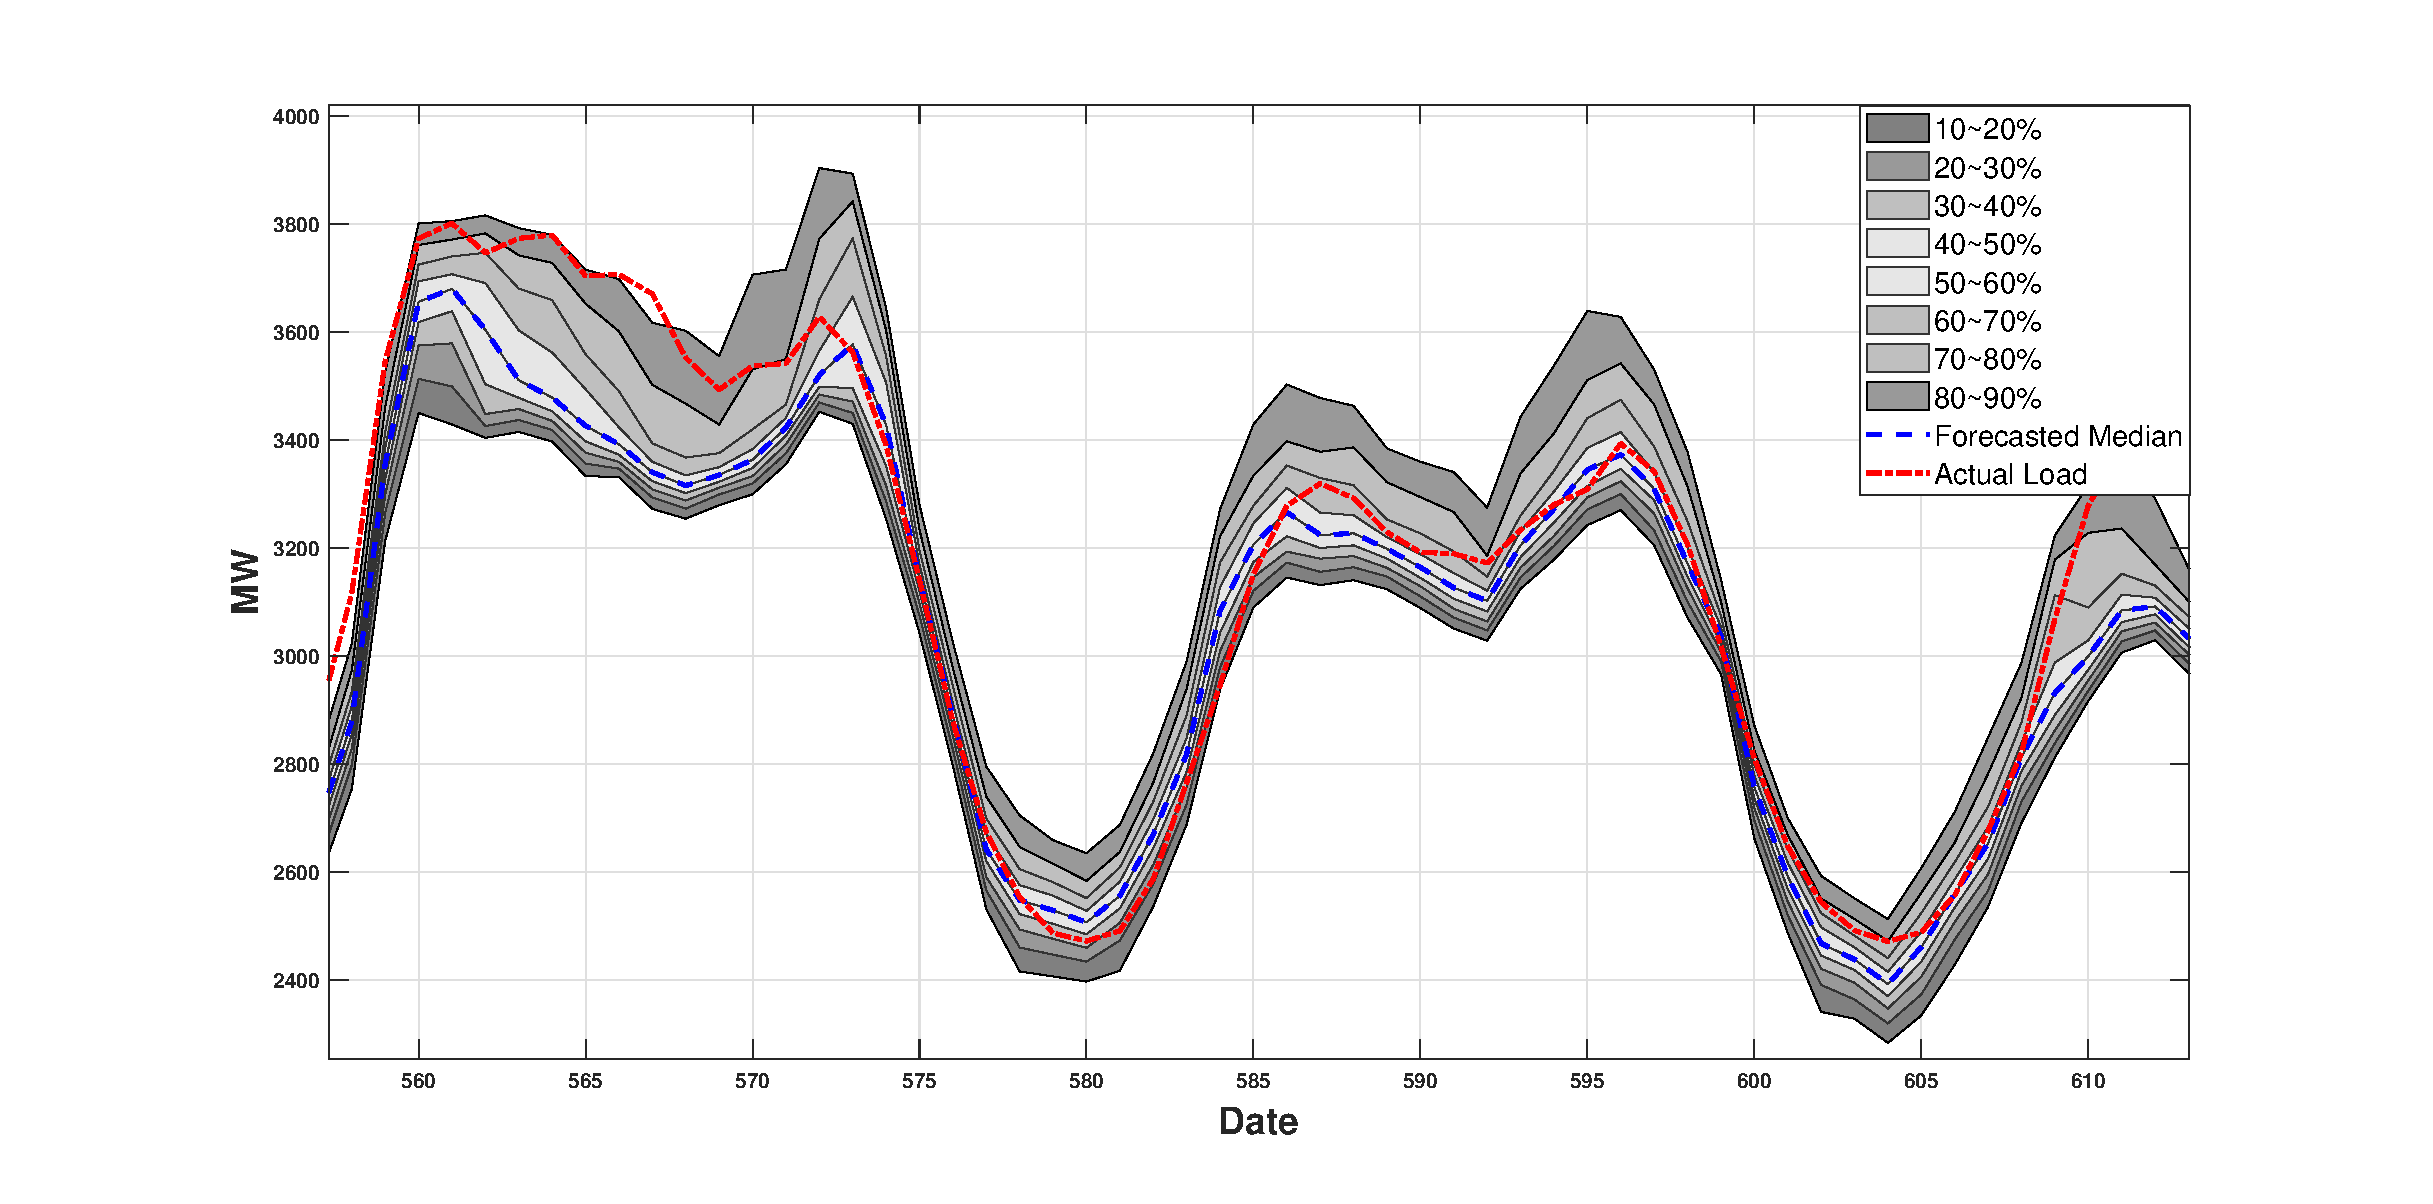
\includegraphics[width=3.5in]{prob.eps}
%\caption{Gaussian Mixture figures with overlapped distributions}
%\label{fig:1}       % Give a unique label
%\end{figure}

\section{Cost Allocation}
\textcolor{red}{With the arrival of the modern electricity market, the cost allocating method of public-use facilities such as power transmission lines are becoming more complicated~\cite{Kirschen2018}. For example, in the past, the cost allocation of power transmission lines were carried out by calculating the amount of flow at each plant based on the peak time~\cite{shahide}. However, revenue from the power system not only arises from increased flow, but also directly or incidentally, such as increased system stability and flexibility. This approach is inefficient and incurring unnecessary costs, although it may be the fairest way to examine all structures that generate revenue in many ways and assess contributions. Thus, today's cost allocation approach have become more complex and equitable, such as a calculating network usage using impedance~\cite{conejo2007z}, an AC power flow Sensitivities~\cite{chaitusaney2002ac}, and a game theory~\cite{zolezzi2002}.}

\subsection{Cooperative Game Theory}
In this paper, we use \textit{cooperative game theory} as a cost allocation method based on benefit. Generally, game theory is divided into two. One is \textit{cooperative game theory} (CGT) and the other is \textit{non-cooperative game theory} (NCGT). NCGT do not seek collective gain through discussion or cooperation between the parties, but consider probabilistic value according to personal choice. The CGT can discussion each other. Thus, interested parties form aggregation called \textit{coalition}, pursue common benefit. Because of characteristic that participants can discussion, it can deduce more accurate result~\cite{zolezzi2002}. The possibility of discussion should be carried out with the game theory considering the combination of participants. Progressing the game theory in all cases can reveal the contribution of each participant in the game, enabling intrinsic characteristics. The structural features of the CGT used in the paper are as follows:



%%\begin{figure}[t!]
%\centering
%  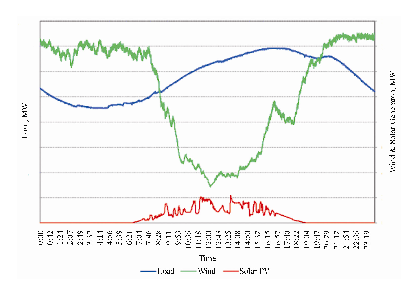
\includegraphics[width=3.5in, height=2.5in]{fig1.eps}
%\caption{Performance with respect to the sampling ranges}
%\label{fig:1}       % Give a unique label
%%\end{figure}











\subsection{Distribution Expansion}













\newpage
\subsubsection{Core}
Core which is the concept expanded \textit{Pareto efficiency} includes feasible set by some axioms. 
\begin{equation}
\sum\limits_{i\in{N}} x_{i} = \textit{v(N)}
\end{equation}
\textit{N} is the universal set that includes all participants. \textit{v(N)} is the coalition function, represent the worth set has. The first means that all benefit is allocated to all participants. And this equation is divided two inequalities.
\begin{equation}
\sum\limits_{i\in{N}} x_{i} \geq v(N)
\end{equation}
Second equation means feasibility. The participants can't allocate more than they produce.
\begin{equation}
\sum\limits_{i\in{S}} x_{i} \geq v(S)
\end{equation}
where \textit{S} is the subset of \textit{N} and means coalition. The last axiom is that the participants in coalition should get pay-off at least they produce.
The \textit{Core} solves the problem using optimization about this axioms. However, if you proceed optimization for the \textit{Core}, it can  appear several value. To allocate clearly, it needs the unique. Thus, the \textit{Nucleolus} is introduced.

\subsubsection{Nucleolus}
\textit{Nucleolus} is the concept expanded at the \textit{Core}. In \textit{Nucleolus}, the focus of the optimization is set to minimizing the worst inequity. To satisfy this, the \textit{excess} is adopted, \textit{excess} represent the difference of worth and sum of pay-off in coalition:
\begin{equation}
e(x,S) = v(S) - \sum\limits_{i\in{S}} x_i
\end{equation}

\subsubsection{Optimization}
When the worth function was set, proceed the optimization . The optimization proceed is as follows.
\begin{center}
Max $\varepsilon$ \; \; \; \; \;\;\;\;\;\;\;\;\;
\end{center}
\begin{center}
\;\;\; $x_i \geq B(i) + \varepsilon$
\end{center}
\begin{center}
$X_i(s) \geq B_i(s) + \varepsilon$
\end{center}
\begin{center}
$\sum\limits_{i\in{S}} x_i = B(N)$ \;\;\;\;
\end{center}

Except for \textit{excess}, all of them is constraints for \textit{Core} axioms. Calculate benefits before and after forming coalition and set constraints according to axioms. Constraints for personal just set condition as many as the number of participants, but in coalition should calculate all possible parties. If there are \textit{N} participants in CGT, it set $2^n$-2 coalitions that except when all participants are included and excluded from $2^n$ that can combine all cases. Once proceed optimization, the results come out. Commonly the results may be not unique. In this happen to get unique solution, proceed optimization again. At preceding optimization, decide minimum value for $x_k$(= $\hat{x}_k$) and $\varepsilon$(=$\varepsilon_k$), apply to the equation as follows.

\begin{center}
Max $\varepsilon_2$ \; \; \; \; \; \; \; \;\;\;\;\;\;\;\;
\end{center}
\begin{center}
$x_k$ = $\hat{x}_k$ \; \; \; \; \;
\end{center}
\begin{center}
\;\;\;\;\;\;\;\;$x_i \geq B(i) + \varepsilon_1 + \varepsilon_2$
\end{center}
\begin{center}
\; \; $X_i(s) \geq B_i(s) + \varepsilon_1 + \varepsilon_2$ 
\end{center}
\begin{center}
$\sum\limits_{i\in{S}} x_i = B(N)$  \; \; \; \;\;\;
\end{center}
Repeat this procedure maximum \textit{N}-1 until get unique.



\begin{figure}[h!]
\centering
  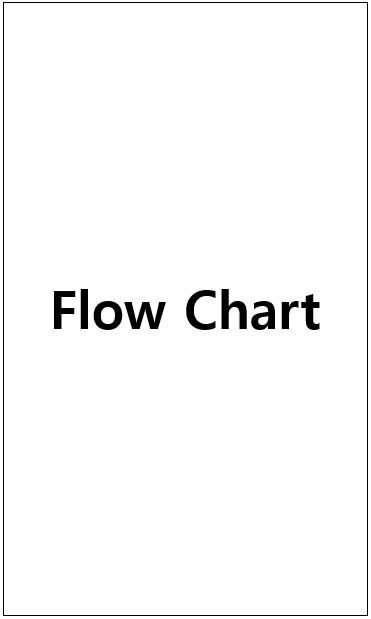
\includegraphics[width=0.8\linewidth]{flow_chart.png}
\caption{flow chart}
\label{flow_chart}
\label{fig:short}
\end{figure}


\subsection{Cost Allocation Methodology}
The cost allocation methodology proposed in this paper consists of a series of steps.
The first step is transmission expansion planning (TEP). The new transmission lines to be built will benefit economically only if the benefits from long-term operations are greater than the cost of construction~\cite{han2020long}. Therefore, to see these economic effects, additional power transmission facilities need to determine the buses and the power transmission capacity that can reduce the incidental costs considered reserve, outage and congestion rents incurred by the system as a whole. Based on this, the following optimization expression is established:
\begin{equation}
\\arg \mathop {\min }\limits_{\zeta (r,s,t)} \sum\limits_{r,s,\in K}^{} {(\mathop \pi \nolimits_\zeta   + \mathop \psi \nolimits_\zeta  } )\
\end{equation}
\;\; Where \textit{K} means set of all nodes in system, \textit{r,s} are selected nodes, \textit{t} is line capacity and $\zeta$ means order pair. $\pi$ of the objective function means the costs incurred when constructing transmission lines on each established node and $\psi$ means the incidental costs incurred in the same situation.

After TEP, the transmission line's node and capacity were determined, the benefit generated between each participant should be calculated. In system congestion situations, system operators direct generators to reduce generation and replace them with regional development for system reliability and stability. Regional generation creates relatively high prices, resulting in an increase in local marginal price (LMP) and overall unnecessary maintenance costs. In this situation, if new power transmission line is installed, the system stability will be increased again and additional power generation of existing power plants will be possible. At the same time, LMP is lowered and maintenance costs are reduced.

Specifically, power plant (PP) benefit from additional generation, transmission system operator (TSO) benefit from more transmission charges and reduced system reliability costs. LSE will able to use electricity that is as cheap as LMP's profit. However, although the TSO and LSE can calculate direct benefit through profit, there is an unreasonable aspect to simply calculate benefit through power generation growth for PP. 

Even if the generation has increased, it is not possible to require high cost allocating to the plant if the utilization rate of the power transmission line is low. to compensate for this, the plant calculates the gain of the increase in power generation over the newly constructed lines by multiplying the increase in power generation power transfer distribution factors (PTDF).

Finally, based on the benefits calculated in the previous step, proceed  a calculation considering all coalition. \textit{\textbf{S}(${\bf{S}} \in {{\bf{R}}^{n}}$)} is the universal set which include all participants that have revenue structure. The first described CGT optimization expression is represented by a matrix form:
\begin{equation}
\begin{array}{l}
\max \varepsilon \\
\;\;\;\;\; {\bf{X}} \ge {\bf{\Lambda }} \cdot {\bf{{\rm \textbf{B}}}} + \varepsilon \\
\sum\limits_{i \in S} {\mathop x\nolimits_i  = B(S)}
\end{array}
\end{equation}

where \textbf{X} has ${2^n} \times 1$ dimension, means the value allocated according to each coalition. ${\bf{\Lambda }}$ and \textbf{B} mean whether to participate and benefit each element respectively. Solving the given optimization results in a allocate value for each participant, and the final cost allocating is derived by converting the share value into a percentage and then multiplying the cost to be allocated. 
\begin{equation}
\nu ({x_i}) = \frac{{{x_i}}}{{\sum x }} \times TC\
\end{equation}
$\nu$ means allocated cost and TC means total cost that should be allocated.

\section{Simulation}
In this section, we proceed numerical experiments on a mid-term forecasting and cost allocation assuming a transmission system for specific zone.

\subsection{Forecasting Architecture}
 For variable selection, we used to build proper regression model, we first tested point forecasting performance. We compared the performance by two different direction. First by cross-validation performance of given training data we tried to find best parameter of regression model. Also in order to confine the scope of usage of given observations, performance of given training data was constructed by iteration of adding data set.  Being based One year ahead observations from the target month and a year when the average demand and temperature were similar to right before the target month, training data were constructed by adding some yearly data.
After building learning model, we fed test data altering weather data for 1000 thousand number of scenario. Then we have 1000 load forecasting observations and 9000 observations for quantile regression each hour. To present load distribution KDE method is used. %Whole forecasting process is described in Fig~\ref{} 

In each process of generating scenario and distribution fitting we set different methods to compare the performance. For sampling method we made distribution of DB and DP independently, considering hourly variable and randomly paired each sample and we call this as individual method. We also sampled from hourly joint distribution of DP DB and this is hourly method. Also to compare the method of choosing final load distribution of each hour, we compared KDE to picking up each 9 quantiles from empirical distribution of 1000 observations. 



\subsection{Performance of Hierarchical  Forecasting}



%%% 1. The performance of 
We measure the performance of hierarchical forecasting. In our hierarchical forecasting, we forecast the load of area whose forecasting performance is better than other areas.
However, the performance of hierarchical forecasting was worse than individual forecasting.



%%%% 2. The performance of total vs individua
The second tested technique is used to forecast the total MA and NE-ISO. First, we forecast the load of all individual areas and add them to forecast the NE-ISO. Second, we directly forecast the load of MA and NE-ISO. Finally, the performance of individually forecasting is better than a direct forecasting of a total value.






\subsection{Performance of Forecasting}

 We compared performance of 10 different forecasting model by pinball loss function. Each score is a summation of forecasting loss of 8 different zone, MA and whole ISO NE. As in Table~\ref{t8} model based on testing scenario which considered dependency of two different temperature and hourly correlation and XGboost with KDE showed best performance. GBM quantile regression showed in Fig~\ref{fig:1}.






















\begin{table}[!t]
	\center
	\renewcommand{\arraystretch}{1.2}
	\caption{Forecasting Model Comparisons}
	\label{Ranking}
	\begin{tabular}{| c | c | c | c | c | }
		\hline
		Zone number& Zone Name    & Our Performance  & Benchmark    \\  \hline
		1 & CT	& 97.79 & 98.8     \\ \hline
		2 & ME & 23.31  & 23.88      \\ \hline
		3 & RI & 19.17 & 21.53     \\ \hline
		4 & NH & 29.14 & 29.64      \\ \hline
		5 & WCMASS & 49.5  & 55.25     \\ \hline
		6 & SEMASS & 44.88 & 49.51      \\ \hline
		7 & NEMASS & 70.93 & 73.16     \\ \hline
		8 & MASS & 161.11 & 175.86      \\ \hline
		&ISO NE & 330.4 & 351.70      \\ \hline
	\end{tabular}
\end{table}


\begin{table}[t!]
	\begin{center}
		\caption{Forecasting Accuracy, Profitability and Computational Time of three Probabilistic Solar Power Forecasting Models}
		\label{t8}
		\begin{tabular}{lccc}
		\toprule
			\toprule % <-- Toprule here
			   & \textbf{Proposed} & \multicolumn{2}{c}{\textbf{Benchmarks}} \\ \cmidrule{3-4}    
			   &Two-Stage Prob. & PP&QGB\\
			\midrule % <-- Midrule here
		    Pinball Loss &\textbf{0.245}& 0.300 & 0.258  \\
		    Entropy &3.652 & 4.035 & \textbf{3.612}\\
		    \midrule 
		    DA Revenue (KRW)  &2,071,462  &1,564,340 & 2,321,903 \\
		    RT Penalty (KRW) & 417,755 & 772,181& 743,511\\
		    \textbf{Profit} (KRW) &  \textbf{1,653,707} &  792,158& 1,578,392\\
			\midrule % <-- Midrule here		    
		    Computation time (min) &58.75& \textbf{0.01} & 60.53  \\
		    
		    
		    \bottomrule
			\bottomrule % <-- Bottomrule here
		\end{tabular}
	\end{center}
	\vspace{-0.2in}
\end{table}


% 1. \subsection{Load Forecasting without Temperature}

% 2. Performance of Hourly Separated Individual Model} (Performance about the individual classified models)

% 3. Performance of hierarchical trickle down model

% 4. Performance of averaged temperature scenarios

% 5. Performance of our own total model


%% \subsection{The performance of Averaged Data}
%% ???

%\subsection{Scenario Windows Analysis}
% fill in the blank later

\begin{figure*}[h!]
\centering
  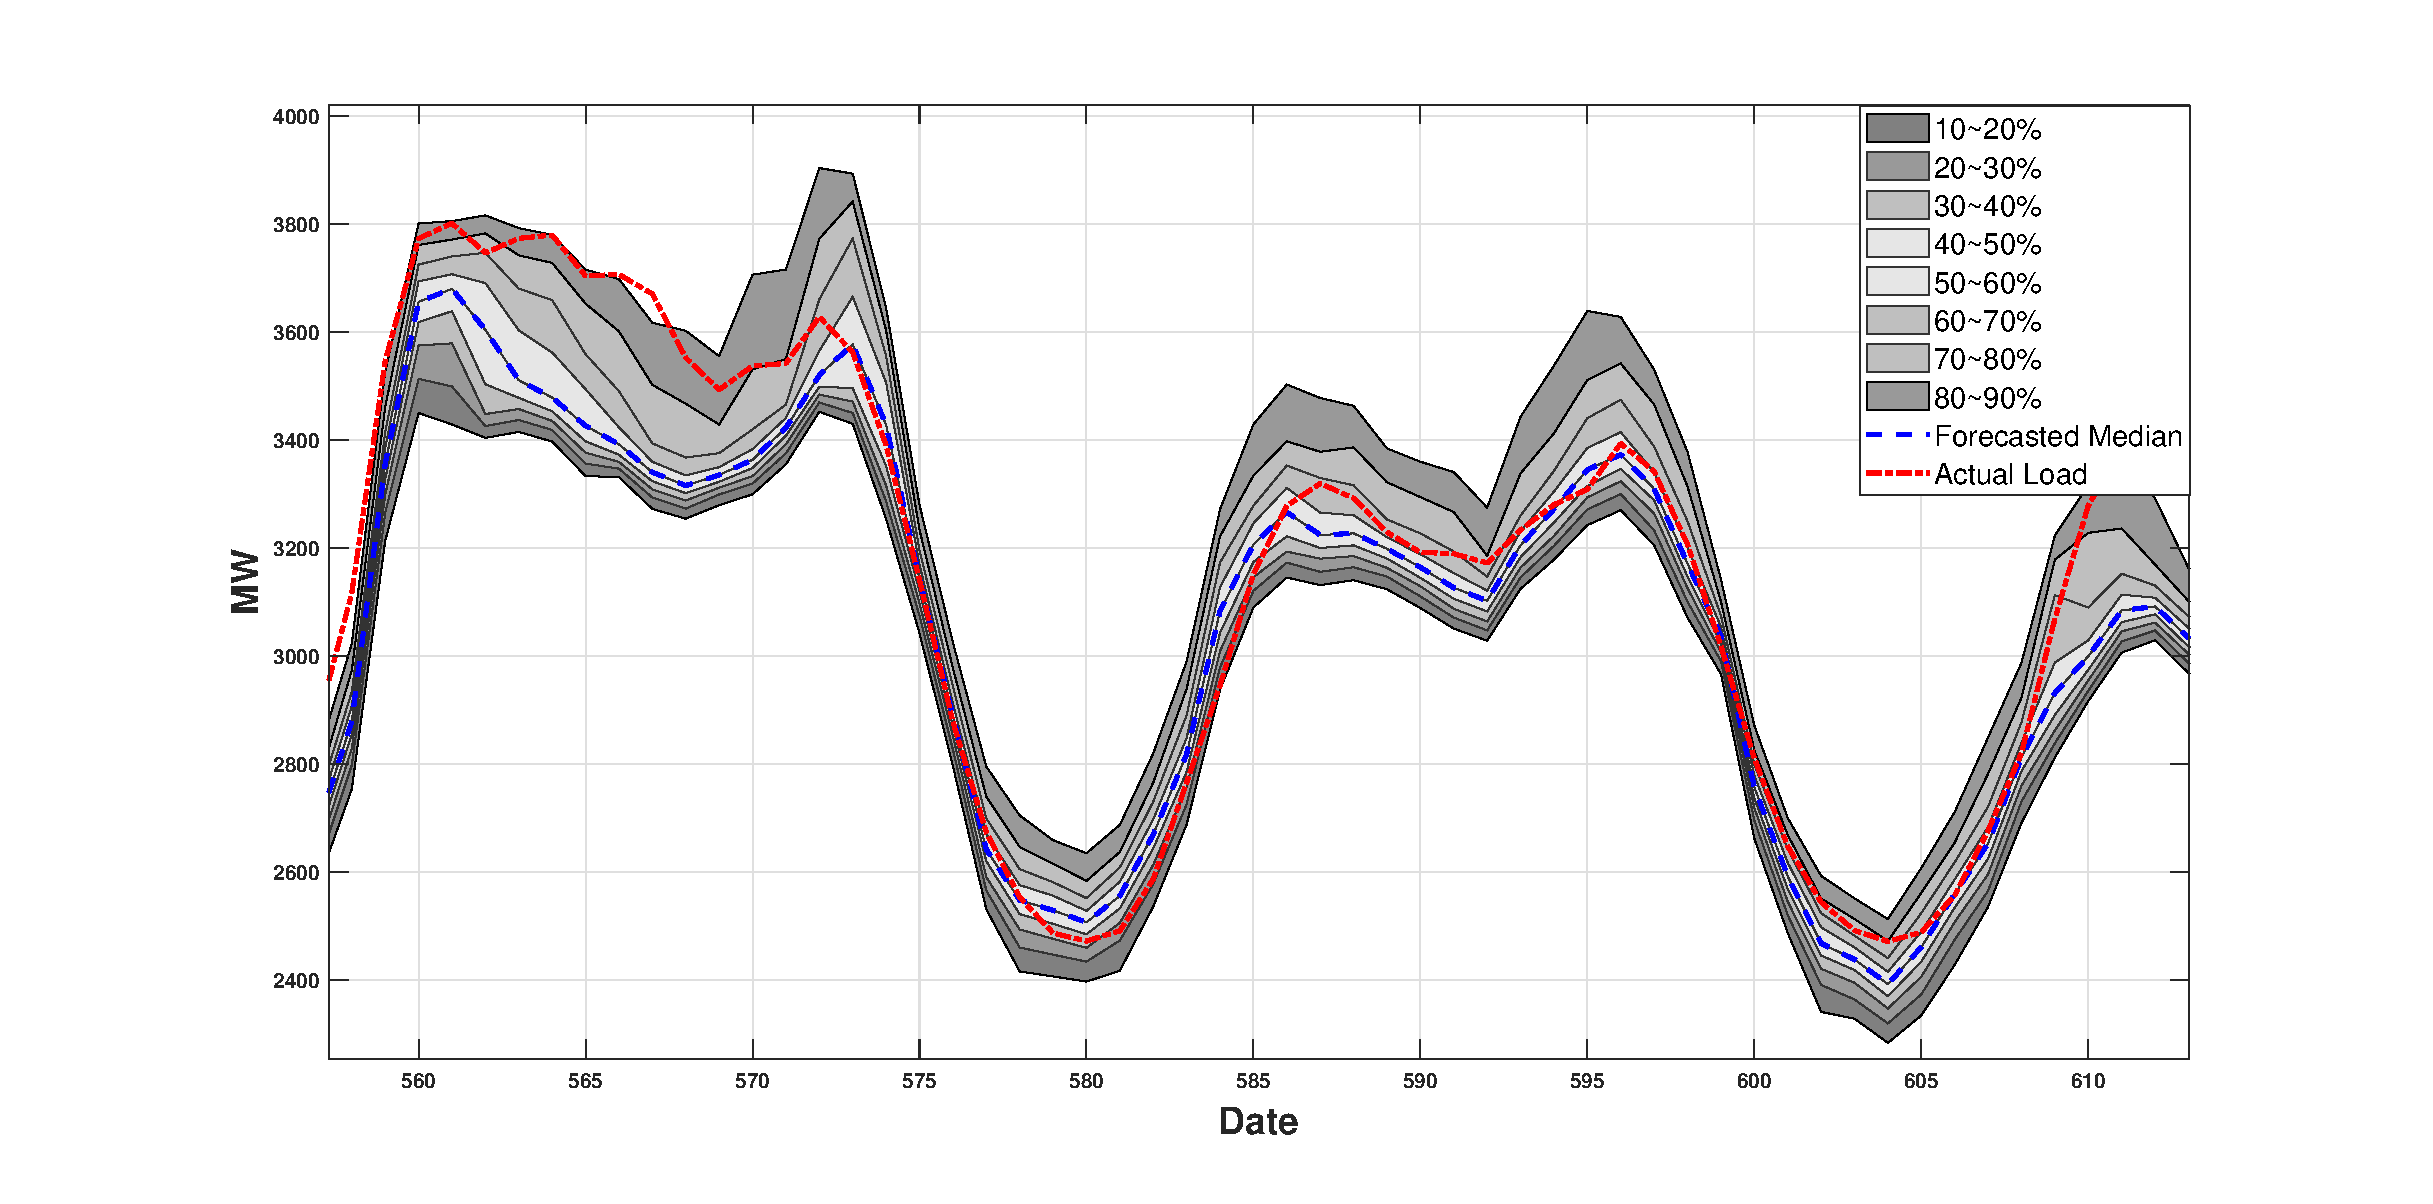
\includegraphics[width=\textwidth]{prob.eps}
\caption{Gaussian Mixture figures with overlapped distributions}
\label{fig:1}       % Give a unique label
\end{figure*}






\subsection{Cost Allocation}
We supposed 8-nodes system which has 8 branches and base plants were located in 1, 2, 3 node respectively (called GEN1, GEN2, GEN3). In addition, each node has a sub generator to prevent imbalance, and the sub generator has a higher power generation cost than the base generations. Fig~\ref{system diagram} shows a entire system and, Table~\ref{table_4} and Table~\ref{Table_5} denote detailed system parameters.

\begin{figure}[h!]
\centering
  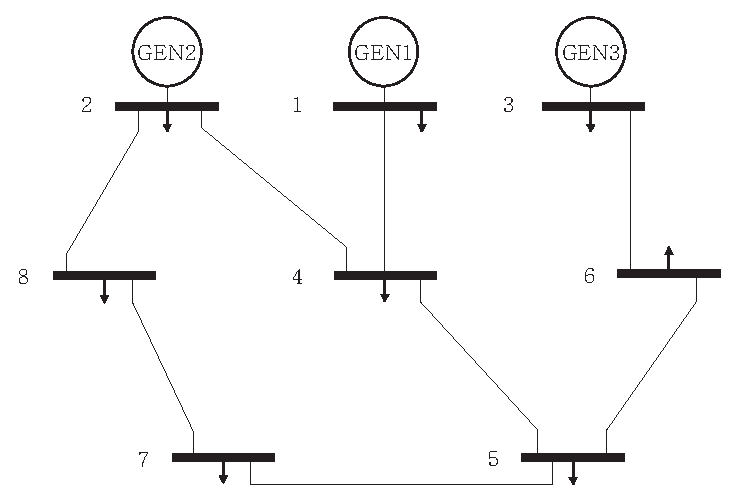
\includegraphics[width=1.0\linewidth]{system_diagram.eps}
\caption{Eight-bus system which describes base generators except sub generators}
\label{system diagram}       % Give a unique label
\end{figure}

\begin{table}[h!]
\centering
\caption{Branch Information}
\label{table_4}
\begin{tabular}{cc | c | c}
\noalign{\smallskip}\noalign{\smallskip}\hline\hline
\multicolumn{2}{c|}{Bus} & \multirow{2}{*}{Rating(MW)} & \multirow{2}{*}{Reactance($\Omega$)}\\
\cline{1-2}
to & from &  &  \\
\hline
1 & 4 & 2000 & 0.0576\\
\hline
4 & 5 & 1500 & 0.0920\\
\hline
5 & 6 & 1500 & 0.1700\\
\hline
3 & 6 & 2000 & 0.0586\\
\hline
6 & 7 & 1500 & 1.008\\
\hline
7 & 8 & 3000 & 0.0720\\
\hline
8 & 2 & 1500 & 0.0625\\
\hline
2 & 4 & 2000 & 0.0780\\
\hline\hline
\end{tabular}
\end{table}

\begin{table}[h!]
\caption{Generator Information}
\label{Table_5}
\centering
\begin{tabular}{c | c c c | c c c}
\hline\hline
\multirow{2}{*}{Gen type} & \multirow{2}{*}{Bus} & \multirow{2}{*}{Labeling} & \multirow{2}{*}{Capacity(MW)} & \multicolumn{3}{|c}{Cost coefficient} \\
\cline{5-7}
&  &  &  & a & b  & c  \\
\hline
\multirow{3}{*}{Base Gen} & 1 &GEN1 & 5000 & 0.1100 & 5.00 & 150\\
\cline{2-7}
& 2 & GEN2 & 8000 & 0.0850 & 1.20 & 600\\
\cline{2-7}
& 3 & GEN3 & 6000 & 0.1225 & 1.00 & 335\\
\hline
\multirow{8}{*}{Sub Gen} & 1 & SUB1 & 2000 & 1.7750 & 10 & 150\\
\cline{2-7}
& 2 & SUB2 & 2000 & 2.2123 & 10 & 150\\
\cline{2-7}
& 3 & SUB3 & 2000 & 1.8548 & 27 & 150\\
\cline{2-7}
& 4 & SUB4 & 2000 & 2.3924 & 50 & 150\\
\cline{2-7}
& 5 & SUB5 & 2000 & 1.9680 & 46 & 100\\
\cline{2-7}
& 6 & SUB6 & 2000 & 1.7879 & 48 & 100\\
\cline{2-7}
& 7 & SUB7 & 2000 & 1.8779 & 10 & 100\\
\cline{2-7}
& 8 & SUB8 & 2000 & 2.0451 & 60 & 100\\
\hline\hline
\end{tabular}
\end{table}

In generator, the GEN2 has cheapest unit price, it maintain a similar generator to others. Because 2-8 transmission line has congestion, GEN2 directly connected to this have no choice but to place a limit on the generating. Simultaneously the LSE use the electricity at higher price, if this status is maintain, losses of total system accumulate.

To decrease system losses, it need additional transmission line. Once proceed TEP optimization, the added transmission line constructed in 2-8 branch. 2-8 branch decrease the LMP and  solve existing congestion. Thus we assume this content and keep experiment.
 
After construction, we calculate the power variance using OPF. According to OPF, the power of GEN2 larger. In contrast the GEN1 and GEN3 decrease for static demand. In this paper, we consider only positive effect of addition line neglect under the zero. The table below is the detailed lineage contents used for OPF.



To decrease system losses, it need additional transmission line. Once proceed TEP optimization, the added transmission line constructed in 2-8 branch. 2-8 branch decrease the LMP and  solve existing congestion. Thus we assume this content and keep experiment.
 
After construction, the OPF for one month is calculated to confirm the \textit{flow} on the expanded transmission line, and the contribution of each generator to the line is calculated by multiplying the PTDF. The benefit of the final generator is calculated by substituting the \textit{flow} of the lines by each generator into the cost curve.

Now that we have obtained the generator benefit, we calculate the benefit of LSE and TSO. The LSE can be calculated through the Lagrangian multiplier of OPF, and the upper limit (850$ \$ $/MW) of the LMP was set prior to line expansion to avoid the dominant responsibility of the LSE dut to the LMP decline. The benefit of TSO can be calculated by the wheeling rate(10$ \$ $/MW). 

Next, the CGT is applied based on the calculated benefits. Five institutions contributed to the cost of expansion transmission lines, with five participants in game theory, and an optimization for this is established.


\begin{align}
&\max \varepsilon \nonumber \\
&\textrm{subject to.} \sum\limits_{\textbf{I} \in S} {\textbf{X}_{I}} \geq \sum\limits_{\textbf{I} \in S} \textbf{B}_{I} + \varepsilon \nonumber \\
&\textit{x}_{i} \geq B_{i} + \varepsilon\\
&\sum\limits_{i=1}^{5} x_{i} = \sum\limits_{i=1}^{5} B_{i} \nonumber
\end{align}

where \textit{S}(\textit{S} $\in$ \textit{R} $\rightarrow$ \textit{R}$^{2^{5}-7}$) means all coalitions and \textbf{I} is possible set in \textit{S}. \textbf{X} is subset of all the coalition and is the number of possible vectors. The constraints were expressed based on the CGT \textit{core} described above.

The results of game theory on the monthly average benefit are as follows:

\begin{table}[h!]
\caption{Cost Allocation Results}
\centering
\begin{tabular}{|c c c c c|}
\hline
GEN1 & GEN2 & GEN3 & LSE & TSO\\[0.5ex]
\hline
0.2774 & 42.0559 & 0 & 49.3645 & 8.3022\\
\hline
\end{tabular}
\end{table}

Thus, Multiplying the ratio shown in the table by the cost of expanding the transmission line finally determines the cost to be shared by each institution.

\section{Conclusion}
  In this paper we proposed novel method to generate NWP scenario for Mid-Term probabilisic load forecasting. We compared the forecasting performance between each scenario making methods. Scenario considering a distribution of 24 hours random variable of each dew point and dry bulb temperature outperformed other methods such as individual sampling or hourly sampling and competition benchmark.
   {We used XGboost for regression model which is most popular machine learning method in recent years for powerful regression ability and low computational load. We also described a method of generating final load distribution from observations of thousand differnet scenarios using kernel density estimation. By this we could get a mathematical form of distribution and also keep original distribution considering each observation.}        





% Can use something like this to put references on a page
% by themselves when using endfloat and the captionsoff option.
\ifCLASSOPTIONcaptionsoff
  \newpage
\fi


\bibliographystyle{IEEEtran}
\bibliography{LoadFore_10}


% biography section
% 
% If you have an EPS/PDF photo (graphicx package needed) extra braces are
% needed around the contents of the optional argument to biography to prevent
% the LaTeX parser from getting confused when it sees the complicated
% \includegraphics command within an optional argument. (You could create
% your own custom macro containing the \includegraphics command to make things
% simpler here.)
%\begin{IEEEbiography}[{\includegraphics[width=1in,height=1.25in,clip,keepaspectratio]{mshell}}]{Michael Shell}
% or if you just want to reserve a space for a photo:




% You can push biographies down or up by placing
% a \vfill before or after them. The appropriate
% use of \vfill depends on what kind of text is
% on the last page and whether or not the columns
% are being equalized.

%\vfill

% Can be used to pull up biographies so that the bottom of the last one
% is flush with the other column.
%\enlargethispage{-5in}



% that's all folks
\end{document}





%% Parametric Approach
%The problem in (\ref{GBMobject} can be seen as to find the set of optimal parameters ${\bf{\hat P}} = \left\{ {{\beta _m},{\alpha _m}} \right\}_1^M$ satisfying
%\begin{equation}
%\label{Parameter}
%{\bf{\hat P}} = \arg \,\mathop {\min }\limits_F \,{E_{{\bf{X}},{\bf{y}}}}\left[ {L({\bf{y}},F({\bf{X}},{\bf{P}}))} \right].
%\end{equation}






